\appendix
%\chapter{First Algorithm}
%\label{app:alg}
%\begin{algorithm}[h]
%	\floatname{algorithm}{Step}
%	\caption{Forward Propagation of Velocity}\label{alg:step1_app}
%	\begin{algorithmic}[1]
	%		\vspace{1mm}
	%		\For{$h=h_1,h_2,h_3,h_4$}
	%		\vspace{1mm}
	%		\State{$V_{bh}=J_{bh,z}\dot{z}+J_{bh,\delta}\dot{\delta}$}
	%		\vspace{1mm}
	%		\State{$V_h=\Ad_{g_{bh}}^{-1}V_b+V_{bh}$}\Comment{Knuckle Rigid-Body Velocity}
	%		\vspace{1mm}
	%		\State{$V_{hw}=J_{hw}\omega$}
	%		\vspace{1mm}
	%		\State{$V_w=V_h+V_{hw}$}\Comment{Rim Rigid-Body Velocity}
	%		\vspace{1mm}
	%		\EndFor
	%		\vspace{1mm}
	%	\end{algorithmic}
%\end{algorithm}
%
%\begin{algorithm}[h]
%	\floatname{algorithm}{Step}
%	\caption{Backward Propagation of Articulated Inertia and Bias}\label{alg:step2_app}
%	\begin{algorithmic}[1]
	%		\vspace{1mm}
	%		\For{$h=h_1,h_2,h_3,h_4$}
	%		\vspace{1mm}
	%		\State{$\hat{M}_w=M_w$}\Comment{Rim Articulated Inertia}
	%		\vspace{1mm}
	%		\State{$\hat{B}_w=-W_{we}+\ad_{V_w}^*M_wV_w$}\Comment{Rim Articulated Bias}
	%		\vspace{1mm}
	%		\State{$\bar{M}_w=\hat{M}_w-\dfrac{\hat{M}_wJ_{hw}J_{hw}^T\hat{M}_w}{J_{hw}^T\hat{M}_wJ_{hw}}$}
	%		\vspace{1mm}
	%		\State{$\bar{B}_w=\hat{B}_w-\dfrac{\hat{M}_wJ_{hw}J_{hw}^T\hat{B}_w}{J_{hw}^T\hat{M}_wJ_{hw}}-\bar{M}_w\ad_{V_{hw}}V_w$}
	%		\vspace{1mm}
	%		\State{$\hat{M}_h= \bar{M}_w$
		%		%\State{$\hat{M}_h= M_h +\bar{M}_w$
			%		}\Comment{Knuckle Articulated Inertia}
		%		\vspace{1mm}
		%		\State{$\hat{B}_h=-W_{he}+\bar{B}_w$
			%			%\State{$\hat{B}_h=-W_{he}+\ad^{*}_{V_h} M_hV_h+\bar{B}_w$
				%			}\Comment{Knuckle Articulated Bias}
			%			\vspace{1mm}
			%			\State{$\bar{M}_h=\hat{M}_h-\dfrac{\hat{M}_hJ_{bh,z}J_{bh,z}^T\hat{M}_h}{J_{bh,z}^T\hat{M}_hJ_{bh,z}}$}
			%			\vspace{1mm}
			%			\State{$\bar{B}_h=\hat{B}_h-\dfrac{\hat{M}_hJ_{bh,z}(J_{bh,z}^T\hat{B}_h-\tau)}{J_{bh,z}^T\hat{M}_hJ_{bh,z}}-\bar{M}_h(\ad_{V_{bh}}V_h-\dot{J}_{bh,z}\dot{z}-\dot{J}_{bh,\delta}\dot{\delta}-J_{bh,\delta}\ddot{\delta})$}
			%			\vspace{1mm}
			%			\EndFor
			%			\vspace{1mm}
			%			\State{$\hat{M}_b=M_b+\displaystyle\sum_h\Ad_{g_{bh}}^*\bar{M}_h\Ad_{g_{bh}}^{-1}$}\Comment{Chassis Articulated Inertia}
			%			\vspace{1mm}
			%			\State{$\hat{B}_b=-W_{be}+\ad_{V_b}^*M_bV_b+\displaystyle\sum_h\Ad_{g_{bh}}^*\bar{B}_h$}\Comment{Chassis Articulated Bias}
			%			\vspace{1mm}
			%	\end{algorithmic}
		%\end{algorithm}
		%
		%\begin{algorithm}[h]
		%	\floatname{algorithm}{Step}
		%	\caption{Forward Propagation of Acceleration}\label{alg:step3_app}
		%	\begin{algorithmic}[1]
			%		\State{$\dot{V}_b=-\hat{M}_b^{-1}\hat{B}_b$}\Comment{Chassis Rigid-Body Acceleration}
			%		\vspace{1mm}
			%		\For{$h=h_1,h_2,h_3,h_4$}
			%		\vspace{1mm}
			%		\State{$\ddot{z}=-\dfrac{J_{bh,z}^T\bigl(\hat{B}_h+\hat{M}_h(\Ad_{g_{bh}}^{-1}\dot{V}_b-\ad_{V_{bh}}V_h+\dot{J}_{bh,z}\dot{z}+\dot{J}_{bh,\delta}\dot{\delta}+J_{bh,\delta}\ddot{\delta})\bigr)-\tau}{J_{bh,z}^T\hat{M}_hJ_{bh,z}}$}
			%		\vspace{1mm}
			%		\State{$\dot{V}_{bh}=\dot{J}_{bh,z}\dot{z}+\dot{J}_{bh,\delta}\dot{\delta}+J_{bh,z}\ddot{z}+J_{bh,\delta}\ddot{\delta}$}
			%		\vspace{1mm}
			%		\State{$\dot{V}_h=\Ad_{g_{bh}}^{-1}\dot{V}_b-\ad_{V_{bh}}V_h+\dot{V}_{bh}$}\Comment{Knuckle Rigid-Body Acceleration}
			%		\vspace{1mm}
			%		\State{$\dot{\omega}=-\dfrac{J_{hw}^T\bigl(\hat{B}_w+\hat{M}_w(\dot{V}_h-\ad_{V_{hw}}V_w)\bigr)}{J_{hw}^T\hat{M}_wJ_{hw}}$}
			%		\vspace{1mm}
			%		\EndFor
			%		\vspace{1mm}
			%	\end{algorithmic}
		%\end{algorithm}
		\section{Smoothing Function}\label{app:smoothing_functions}
		The optimizer, in order to find the solution, calculates several number of derivatives, hence, having differentiable function, possibly of class $C^\infty$, improves the quality of the solution and reduces the simulation time. 
		
		Here is proposed a smooth step function, used to perform comparison between decision variables, that exploits hyperbolic functions. 
		\begin{equation}\label{eq:ifelsesmooth}
			z = \frac{T}{2}\left[1 + \tanh(C\left(x-y\right))\right] + \frac{F}{2}\left[1 - \tanh(C\left(x-y\right))\right],
		\end{equation}
		where $T$ and $F$ represent the asymptotic values of the function when $x>y$ and $x<y$, respectively, while $C$ is a constant used to tune the hardness of the intervention. 
		Supposing to model an absolute value of $x$, setting $T=1$, $F=-1$, and $C=10$, reducing $z$ to depend only on $x$, the function can be expressed as follows:
		\begin{equation}
			\tilde{abs}(x) = z(x)\cdot x.
		\end{equation}
		
		\begin{figure}[h]
			\centering
			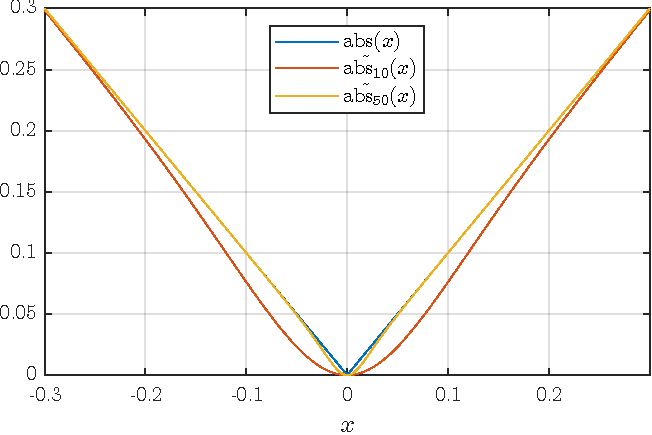
\includegraphics[scale = .8]{Images/Appendices/abs_smooth.pdf}
			\caption{Comparison between non derivable abs function (in blue) and two smooth abs functions (in red and yellow). The subscript on the smooth function indicates the value of the constant $C$, which tunes the hardness of the intervention. Increasing this value leads to a more accurate function, but results in higher derivatives as a drawback.}
			\label{fig:abs_smooth}
		\end{figure}